\documentclass[11pt,a4paper,hidelinks]{article}

\setlength{\headheight}{26pt}

% Packages
\usepackage[left=25mm, right=25mm, top=35mm, bottom=25mm]{geometry} % defines whitespaces on the edges
\usepackage[bottom, hang]{footmisc}
\usepackage{hyperref}             % for \nameref and cite
\usepackage{footnotebackref}      % used for getting back from the footnote to the main text
\usepackage{enumitem}
\usepackage{graphicx}
\usepackage{fancyhdr}
\usepackage{lastpage}
\usepackage[export]{adjustbox}
\usepackage{float}
\usepackage[ngerman]{babel}
\usepackage[ngerman]{datetime}
\usepackage{apacite}
\usepackage[utf8]{inputenc}
\usepackage{listings}
\usepackage{xcolor}
\usepackage{pdfpages}
\usepackage{url}
\usepackage{outlines}
\usepackage{tocloft}
\usepackage[utf8]{inputenc}
\usepackage{amsmath}
\usepackage{mathtools}
\usepackage[acronym]{glossaries}
\usepackage{titlesec}             % for \titleformat
\usepackage{textcomp}             % for \degree sign
\usepackage{gensymb}              % for \degree sign
\usepackage{csvsimple}            % for using csv-files for tables
\usepackage{lscape}               % for landscape mode
\usepackage{parskip}              % inserts space after paragraph automatically
\usepackage{svg}                  % used to include svg with the help of inkscape which converts svg to pdf
\usepackage{wasysym}              % for \diameter symbol
\usepackage{xfrac}                % for \sfrac

\frenchspacing  % Use same space size between words and between sentences

% change section titles' font size
\titleformat*{\section}{\huge\bfseries}
\titleformat*{\subsection}{\LARGE\bfseries}
\titleformat*{\subsubsection}{\Large\bfseries}
\titleformat{\paragraph}[hang]{\large\bfseries}{\theparagraph}{1em}{}
\titleformat{\subparagraph}[hang]{\normalsize\bfseries}{\thesubparagraph}{1em}{}

\definecolor{codegreen}{rgb}{0,0.6,0}
\definecolor{codegray}{rgb}{0.5,0.5,0.5}
\definecolor{codepurple}{rgb}{0.58,0,0.82}
\definecolor{codeorange}{rgb}{1,0.5,0.15}
\definecolor{backcolour}{rgb}{0.9,0.9,0.9}

\lstdefinestyle{mystyle}{
    backgroundcolor=\color{backcolour},
    commentstyle=\color{codegreen},
    keywordstyle=\color{magenta},
    numberstyle=\tiny\color{codegray},
    stringstyle=\color{codepurple},
    basicstyle=\ttfamily\footnotesize,
    breakatwhitespace=false,
    breaklines=true,
    captionpos=b,
    keepspaces=true,
    numbers=left,
    numbersep=5pt,
    showspaces=false,
    showstringspaces=false,
    showtabs=false,
    tabsize=4
}
\lstset{style=mystyle}

\lstset{
    literate={~} {$\sim$}{1}
}

\lstset{%
    breaklines=true,
    breakatwhitespace=true,
}

\DeclarePairedDelimiter\abs{\lvert}{\rvert} % make scalable absolute stripes
\DeclarePairedDelimiter\parenth{(}{)} % make scalable parentheses

\let\phi\varphi{} % change style of \phi sign

\setlength{\parindent}{0mm} % disable paragraph indent

\newdateformat{mydate}{\THEDAY{. }\monthnamengerman[\THEMONTH] \THEYEAR}

\renewcommand{\listfigurename}{}
\renewcommand\contentsname{Inhaltsverzeichnis}
\renewcommand\lstlistingname{Code}

\makeglossaries{}

% Header/Footer Setting
\setlength\footnotemargin{15pt}
\pagestyle{fancy}
\fancyhf{}
\renewcommand{\footrulewidth}{0.4pt} % footer line
\rhead{\textbf{\vUniversity}\\\vModule}
\lhead{\textbf{\vTitle}\\
    Projektarbeit}
\lfoot{\vAuthorFirstName{} \vAuthorLastName}
\cfoot{\mydate\today}
\rfoot{S.~\thepage~/~\pageref{LastPage}}

% Redefine the plain page style, otherwise there is no header and footer for chapter pages
\fancypagestyle{plain}{%
    \fancyhf{}
    \renewcommand{\footrulewidth}{0.4pt} % footer line
    \rhead{\textbf{\vUniversity}\\\vModule}
    \lhead{\textbf{\vTitle}\\
        Projektarbeit}
    \lfoot{\vAuthorFirstName{} \vAuthorLastName}
    \cfoot{\mydate\today}
    \rfoot{S.~\thepage~/~\pageref{LastPage}}
}

\bibliographystyle{apacite}

% Settings for the equation list
\newcommand{\listequationsname}{}
\newlistof{myequations}{equ}{\listequationsname}
\renewcommand{\cftmyequationsaftersnum}{\hfill}
\renewcommand{\cftmyequationspresnum}{\hfill}
\setlength{\cftmyequationsnumwidth}{3.5em}
\newcommand{\myequations}[1]{%
\addcontentsline{equ}{myequations}{\protect\numberline{\theequation}#1}\par}

\newcommand{\mytable}[4]
{
    \centering
    \begin{tabular}{#1}\hline%
        #2 \\ \hline
        \csvreader[
            separator=semicolon,
            head to column names,
            late after line=\\,
        ]{#4}{}{#3}
        \hline
    \end{tabular}
}


% Variables
\newcommand{\vTitle}{DIY Optische ToF Distanzmessung}
\newcommand{\vModule}{CAS Sensorik und Sensor Signal Conditioning}
\newcommand{\vAuthorFirstName}{Matthias Schär,}
\newcommand{\vAuthorLastName}{Timon Burkard}
\newcommand{\vUniversity}{OST -- Ostschweizer Fachhochschule}
\newcommand{\vDegree}{CAS Sensorik und Sensor Signal Conditioning}
\newcommand{\vSemester}{HS24}
\newcommand{\vProfessor}{Prof. Guido Keel, Michael Lehmann}
\newcommand{\vCity}{Rapperswil}
\newcommand{\vAbstract}{Die vorliegende Projektarbeit befasst sich mit der Entwicklung eines\dots}

% Acronyms
\newacronym{pcb}{PCB}{Printed Circuit Board}
\newacronym{tof}{ToF}{Time of Flight}
\newacronym{diy}{DIY}{Do It Yourself}
\newacronym{tdc}{TDC}{Time to Digital Converter}
\newacronym{tia}{TIA}{Trans-Impedance Amplifier}

\begin{document}

\title{\vspace{-40pt}\begin{huge}\textbf{\vTitle}\end{huge}\\
\ \\ \vModule}
\author{\\\\\textbf{\vAuthorFirstName{} \vAuthorLastName}\\
    \vUniversity{}\\
    \\\\}

\date{\mydate\today}
\maketitle\thispagestyle{empty}  % removes footer from first page

\vspace{35pt}

\begin{figure}[H]
    \centering
    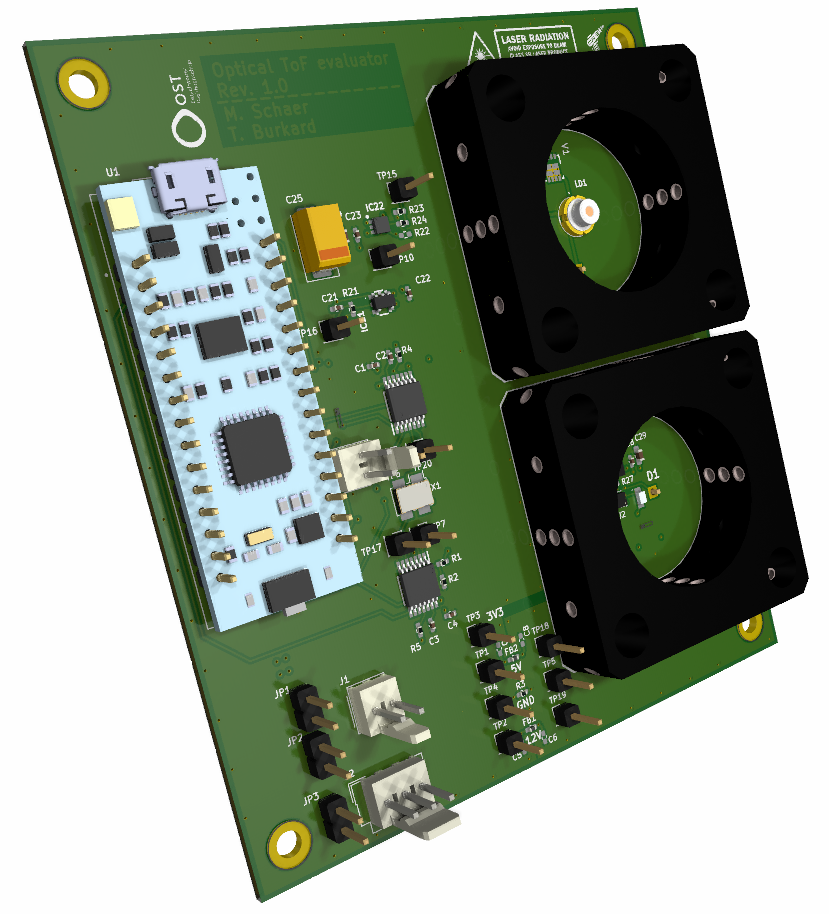
\includegraphics[width=0.6\textwidth]{graphics/cover_picture.png}
\end{figure}

\vspace{30pt}

\begin{figure}[H]
    \centering
    \begin{minipage}[b]{0.3\textwidth}
        \includesvg[width=\textwidth]{graphics/OST_Logo.svg}\label{fig:OST_Logo}
    \end{minipage}
\end{figure}

\pagebreak

\thispagestyle{empty}

\textbf{}
\vspace{5mm}

\begin{flushleft}
    \textbf{\large{\vModule{} an der \vUniversity{}}}
\end{flushleft}

\begin{flushleft}
    \begin{small}
        \begin{tabular}{@{}lll}
            \\
            \textbf{Titel}                 & & \textbf{\vTitle}\\
            \\
            \textbf{Diplomandin/Diplomand} & & \textbf{\vAuthorFirstName{} \vAuthorLastName}\\
            \\
            \textbf{Studiengang}           & & \textbf{\vDegree}\\
            \\
            \textbf{Semester}              & & \textbf{\vSemester}\\
            \\
            \textbf{Dozentin/Dozent}       & & \textbf{\vProfessor}\\
        \end{tabular}
    \end{small}
\end{flushleft}

\vspace{10mm}

% abstracts
\begin{flushleft}
    \begin{small}
        \textbf{Abstract} \\
        \vAbstract{}
        \vspace{15mm}
    \end{small}
\end{flushleft}

% copyright
\begin{flushleft}
    \begin{small}
        Ort, Datum\hspace{30mm}\vCity, \date{\mydate\today} \\
        \textbf{\textcopyright\hspace{1mm}\vAuthorFirstName{} \vAuthorLastName, \vUniversity{}}
    \end{small}
\end{flushleft}

\mbox{}
\vfill

\noindent\makebox[\linewidth]{\rule{\textwidth}{1pt}}
% copyright notice
\begin{flushleft}
    \begin{small}
        Alle Rechte vorbehalten. Die Arbeit oder Teile davon dürfen ohne schriftliche Genehmigung der Rechteinhaber weder in irgendeiner Form reproduziert noch elektronisch gespeichert, verarbeitet, vervielfältigt oder verbreitet werden.\\~\\
        Sofern die Arbeit auf der Website der Ostschweizer Fachhochschule online veröffentlicht wird, können abweichende Nutzungsbedingungen unter Creative-Commons-Lizenzen gelten. Massgebend ist in diesem Fall die auf der Website angezeigte Creative-Commons-Lizenz.
    \end{small}
\end{flushleft}

\pagebreak

\section*{Inhaltsverzeichnis}
\vspace{-25pt}
\renewcommand*\contentsname{}
\tableofcontents

\pagebreak

\section*{Abkürzungsverzeichnis}
\vspace{-25pt}
\printglossary[type=\acronymtype,title={}]

\pagebreak

\section*{Abbildungsverzeichnis}
\vspace{-25pt}
\renewcommand{\listfigurename}{}
\listoffigures

\pagebreak

\section*{Formelverzeichnis}
\vspace{-25pt}
\listofmyequations{}

\pagebreak

\section*{Tabellenverzeichnis}
\vspace{-25pt}
\renewcommand{\listtablename}{}
\listoftables

\pagebreak

\section*{Codeverzeichnis}
\vspace{-33pt}
\renewcommand{\lstlistlistingname}{}
\lstlistoflistings{}

\pagebreak


%%%%%%%%%%%%%%%%%%%%%% CONTENT START %%%%%%%%%%%%%%%%%%%%%%

\section{Einleitung}

Bei dieser Projektarbeit geht es darum ein \acrfull{diy} optisches \acrfull{tof} Distanzmesssystem aufzubauen. Dazu soll ein \acrfull{tdc} verwendet werden.

\dots

\pagebreak

\section{Theorie}

\subsection{Time of Flight}

Bei \acrshort{tof} handelt es sich um \dots

\pagebreak

\subsection{Photostrom}

Zur Berechnung des theoretisch zu erwartenden Photostrom wird von einer Distanz zur Wand von $10~m$ ausgegangen.

Der Laserstrahl gehe idealisiert mit $0\degree$ zur Wand und werde dort uniform Halbkugel-förmig gestreut. In der Realität wird sich die Streuung nicht uniform verteilen, sondern in der Mitte stärker konzentriert sein. Die folgende Berechnung zeigt also den worst case.

Die Berechnung der empfangenen Strahlungsleistung, der Strahlungsintensität, dem Raumwinkel und dem Photostrom sind in Formel~\ref{eq:pin}, \ref{eq:ie}, \ref{eq:omega} bzw. \ref{eq:iph} gezeigt.

\begin{equation}\label{eq:pin}
    P_{in} = E_e \cdot A = \frac{I_e}{r^2} \cdot A
\end{equation}
\myequations{Eintreffende Lichtleistung}

\begin{equation}\label{eq:ie}
    I_e = \frac{P_{out}}{\Omega}
\end{equation}
\myequations{Strahlungsintensität}

\begin{equation}\label{eq:omega}
    \Omega = \frac{4\cdot \pi \cdot 0.5}{d}
\end{equation}
\myequations{Raumwinkel}

\begin{equation}\label{eq:iph}
    I_{ph} = S \cdot P_{in}
\end{equation}
\myequations{Photostrom}

\subsubsection{Berechnung mit RLD94PZJ5 und BPV23NF}

Ersten Berechnungen wurden mit der Laserdiode RLD94PZJ5 \cite{rohm2020rld94pzj5_datasheet} und der Photodiode BPV23NF \cite{vishay2024bpv23nf_datasheet} durchgeführt.

Die relevanten Werte aus den Datenblättern sind in Formel~\ref{eq:rld94pzj5_num} und \ref{eq:rbpv23nf_num} aufgelistet.

\begin{equation}\label{eq:rld94pzj5_num}
    P_{out} = 285~mW
\end{equation}
\myequations{Werte des RLD94PZJ5}

\begin{equation}\label{eq:rbpv23nf_num}
    \begin{split}
        A &= 4.4~mm^2\\
        S &= 0.6~\frac{A}{W}
    \end{split}
\end{equation}
\myequations{Werte des BPV23NF}

Diese Werte eingesetzt in Formel~\ref{eq:ie}, \ref{eq:pin} und \ref{eq:iph} ergibt die Resultate in Formel~\ref{eq:rld94pzj5_rbpv23nf_num}.

\begin{equation}\label{eq:rld94pzj5_rbpv23nf_num}
    \begin{split}
        I_e    &= \frac{P_{out}}{\Omega} = \frac{285~mW}{\frac{4\cdot \pi \cdot 0.5}{d}} = \frac{285~mW}{\frac{4\cdot \pi \cdot 0.5}{10~m}} = 45~\frac{mW}{sr}\\
        P_{in} &= \frac{I_e}{r^2} \cdot A = 45~\frac{mW}{sr} \cdot 4.4~mm^2 = 2~nW\\
        I_{ph} &= S \cdot P_{in} = 0.6~\frac{A}{W} \cdot 2~nW = 1.2~nA
    \end{split}
\end{equation}
\myequations{Nummerische Resultate mit RLD94PZJ5 und BPV23NF}

\subsubsection{Berechnung mit RLD65NZX1 and NJL6401R-3}

Die Laserdiode RLD94PZJ5 hat im Bezug auf diese Projektarbeit zwei Nachteile: Sehr hohe Leistung, welche für das menschliche Auge gefährlich werden kann und ein Wellenlängenbereich, der für das menschliche Auge nicht sichtbar ist.

Aus diesen Gründen wurde eine zweite Laserdiode evaluiert: RLD65NZX1 \cite{rohm2019rld65nzx1_datasheet}. Gepaart wird sie mit der Photodiode NJL6401R-3 \cite{jrc2014njl6401r3_datasheet}. Die folgenden Berechnungen wurden basierend auf diesen beiden Komponenten durchgeführt.

Die relevanten Werte aus den Datenblättern sind in Formel~\ref{eq:rld65nzx1_num} und \ref{eq:njl6401r3_num} aufgelistet.

\begin{equation}\label{eq:rld65nzx1_num}
    P_{out} = 10~mW
\end{equation}
\myequations{Werte des RLD65NZX1}

\begin{equation}\label{eq:njl6401r3_num}
    \begin{split}
        A &= 0.7~mm \cdot 0.7~mm = 0.49~mm^2\\
        S &= 0.42~\frac{A}{W}
    \end{split}
\end{equation}
\myequations{Werte des NJL6401R-3}

Diese Werte eingesetzt in Formel~\ref{eq:ie}, \ref{eq:pin} und \ref{eq:iph} ergibt die Resultate in Formel~\ref{eq:rld65nzx1_njl6401r3_num}.

\begin{equation}\label{eq:rld65nzx1_njl6401r3_num}
    \begin{split}
        I_e    &= \frac{P_{out}}{\Omega} = \frac{10~mW}{\frac{4\cdot \pi \cdot 0.5}{d}} = \frac{10~mW}{\frac{4\cdot \pi \cdot 0.5}{10~m}} = 1.6~\frac{mW}{sr}\\
        P_{in} &= \frac{I_e}{r^2} \cdot A = 45~\frac{mW}{sr} \cdot 0.49~mm^2 = 8~pW\\
        I_{ph} &= S \cdot P_{in} = 0.42~\frac{A}{W} \cdot 8~pW = 3.3~pA
    \end{split}
\end{equation}
\myequations{Nummerische Resultate mit RLD65NZX1 and NJL6401R-3}

\pagebreak

\subsection{Transimpedanzverstärker}

Bei einem \acrfull{tia} handelt es sich um \dots

\pagebreak

\section{Umsetzung}

\subsection{Firmware}

\pagebreak

\subsection{Schaltungen}

\subsubsection{Selective Input Voltage}

Abbildung~\ref{fig:selective_input_voltage} zeigt die Beschaltung zur Selektion der Speisung.

\begin{figure}[H]
    \centering
    \includegraphics[page=2, trim=80 590 750 50, clip, width=0.9\textwidth]{attachments/schematic.pdf}
    \caption{Selective Input Voltage}\label{fig:selective_input_voltage}
\end{figure}

Für die Speisung des Nucleo-Boards bestehen die folgenden Möglichkeiten:

\begin{itemize}
    \item 5V von USB-Buchse
    \item 5V von externem Power-Supply (JP1 + JP2)
    \item 12V von externem Power-Supply (JP3)
\end{itemize}

Siehe dazu auch Kapitel~\ref{sec:schematic_nucleo}.

Für die Speisung der 5V-Elektronik bestehen die folgenden Möglichkeiten:

\begin{itemize}
    \item 5V von Nucleo-Board (JP1)
    \item 5V von externem Power-Supply (JP2)
    \item 12V von externem Power-Supply via Nucleo-Board (JP1 + JP3)
\end{itemize}

Für die Speisung der Photodiode bestehen die folgenden Möglichkeiten:

\begin{itemize}
    \item 5V von 5V-Elektronik (SW2 Position 3)
    \item 12V von externem Power-Supply (SW2 Position 1)
\end{itemize}

Siehe dazu auch Kapitel~\ref{sec:schematic_photo_receiver}.

\subsubsection{Nucleo Board}\label{sec:schematic_nucleo}

Die Beschaltung des NUCLEO-F042K6 Boards \cite{st2024nucleof042k6_usermanual} ist in Abbildung~\ref{fig:nucleo_board} gezeigt.

\begin{figure}[H]
    \centering
    \includegraphics[page=2, trim=530 580 300 50, clip, width=0.9\textwidth]{attachments/schematic.pdf}
    \caption{Nucleo Board}\label{fig:nucleo_board}
\end{figure}

\subsubsection{TDC Electrical Signal}

Die Beschaltung des TDC7200 \cite{ti2016tdc7200_datasheet} für den elektrischen Teil ist in Abbildung~\ref{fig:tdc_ele_signal} gezeigt.

\begin{figure}[H]
    \centering
    \includegraphics[page=2, trim=80 330 750 310, clip, width=0.9\textwidth]{attachments/schematic.pdf}
    \caption{TDC Electrical Signal}\label{fig:tdc_ele_signal}
\end{figure}

\subsubsection{TDC Optical Signal}

Die Beschaltung des TDC7200 \cite{ti2016tdc7200_datasheet} für den optischen Teil ist in Abbildung~\ref{fig:tdc_opt_signal} gezeigt.

\begin{figure}[H]
    \centering
    \includegraphics[page=2, trim=530 330 300 310, clip, width=0.9\textwidth]{attachments/schematic.pdf}
    \caption{TDC Optical Signal}\label{fig:tdc_opt_signal}
\end{figure}

\subsubsection{Oscillator For TDCs}

Die Beschaltung des Oszillators für die beiden \acrshort{tdc} ist in Abbildung~\ref{fig:oscillator_tdc} gezeigt.

\begin{figure}[H]
    \centering
    \includegraphics[page=2, trim=80 90 930 550, clip, width=0.45\textwidth]{attachments/schematic.pdf}
    \caption{Oscillator for TDCs}\label{fig:oscillator_tdc}
\end{figure}

\subsubsection{Power Supply Separation}

Für die Beschaltung der Photodiode, inkl. \acrshort{tia} und Komparator, macht es Sinn eine Spannungsversorgung mit möglichst wenig Rauschen zu haben.

Dazu wurde die Separierung vorgenommen, welche in Abbildung~\ref{fig:power_supply_separation} dargestellt ist.

\begin{figure}[H]
    \centering
    \includegraphics[page=2, trim=260 90 640 550, clip, width=0.7\textwidth]{attachments/schematic.pdf}
    \caption{Power Supply Separation}\label{fig:power_supply_separation}
\end{figure}

\subsubsection{Laser Driver}

Die Laser Diode RLD65NZX1 \cite{rohm2019rld65nzx1_datasheet} wird mittels Lasertreiber LMG1025-Q1 \cite{ti2024lmg1025q1_datasheet} und NexFET \cite{ti2016csd17578q3a_datasheet} angesteuert. Für die Generierung eines kurzen Pulses (0.5 \dots 100~ns) wurde mittels Hochpass und AND-Gatter \cite{diodes202074lvc1g08q_datasheet} implementiert. Siehe dazu Abbildung~\ref{fig:laser_driver}.

\begin{figure}[H]
    \centering
    \includegraphics[page=3, trim=100 520 550 60, clip, width=0.9\textwidth]{attachments/schematic.pdf}
    \caption{Laser Driver}\label{fig:laser_driver}
\end{figure}

\subsubsection{Photo Receiver}\label{sec:schematic_photo_receiver}

Um den Photostrom der Photodiode NJL6401R \cite{jrc2014njl6401r3_datasheet} zu verstärken und in eine Spannung umzuwandeln, wurde mit dem Operationsverstärker OPA858 \cite{ti2018opa858_datasheet} ein Transimpedanzverstärker aufgebaut. Der Ausgangs des Transimpedanzverstärkers geht auf den Komparator TLV3501 \cite{ti2016tlv3501_datasheet}, um das STOP-Signal für den \acrshort{tdc} zu generieren. Siehe dazu Abbildung~\ref{fig:photo_receiver}.

\begin{figure}[H]
    \centering
    \includegraphics[page=3, trim=100 240 600 340, clip, width=0.9\textwidth]{attachments/schematic.pdf}
    \caption{Photo Receiver}\label{fig:photo_receiver}
\end{figure}

\subsubsection{Decoupling Capacitors}

Die Beschaltung der Entkopplungs-Kondensatoren ist in Abbildung~\ref{fig:decoupling_capacitors} dargestellt.

\begin{figure}[H]
    \centering
    \includegraphics[page=3, trim=100 60 650 630, clip, width=0.9\textwidth]{attachments/schematic.pdf}
    \caption{Decoupling Capacitors}\label{fig:decoupling_capacitors}
\end{figure}

\pagebreak

\subsection{Layout}

In diesem Kapitel werden die \acrshort{pcb}-Layouts dokumentiert.

\subsubsection{Kupfer-Layer}

\begin{figure}[H]
    \centering
    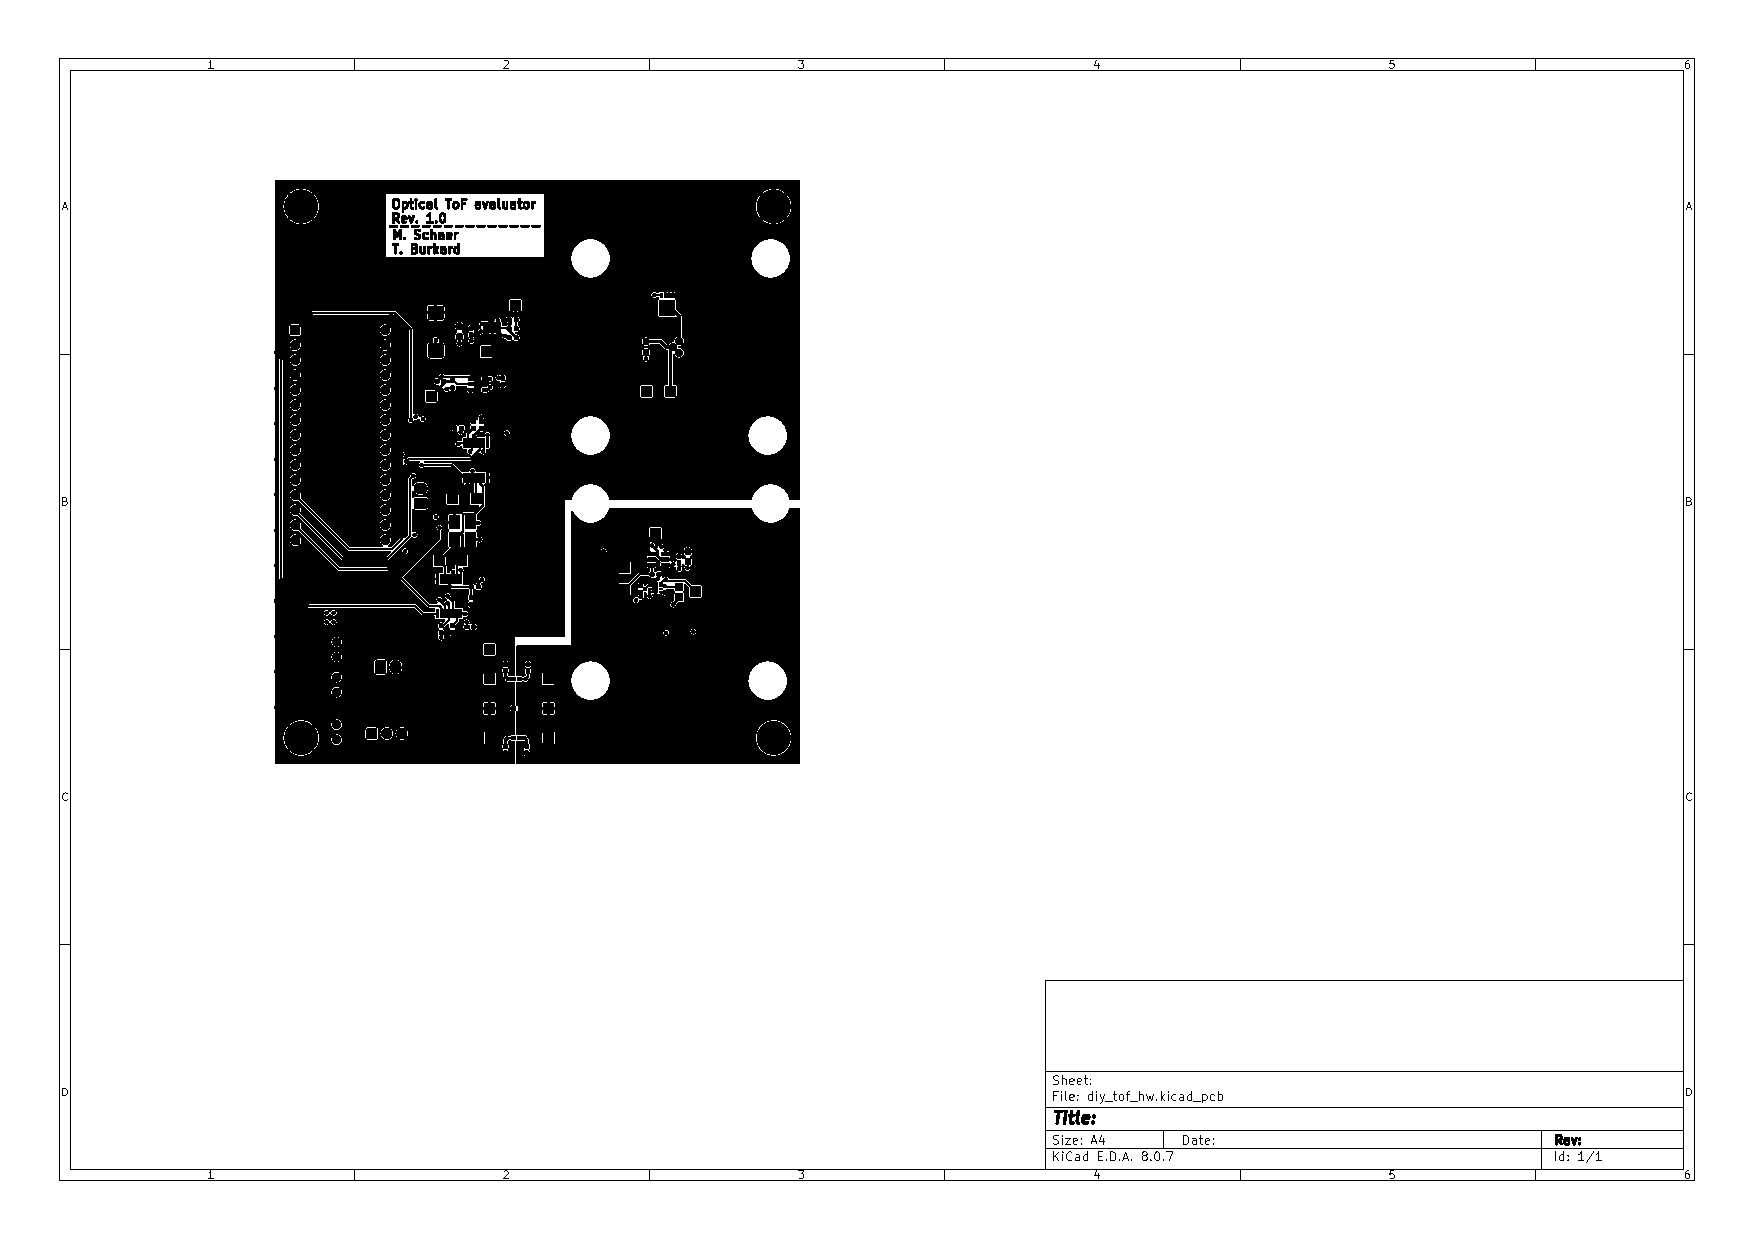
\includegraphics[trim=130 220 450 80, clip, width=0.6\textwidth]{attachments/pcb_F_Cu.pdf}
    \caption{PCB Layout Top}\label{fig:pcb_f_cu}
\end{figure}

\begin{figure}[H]
    \centering
    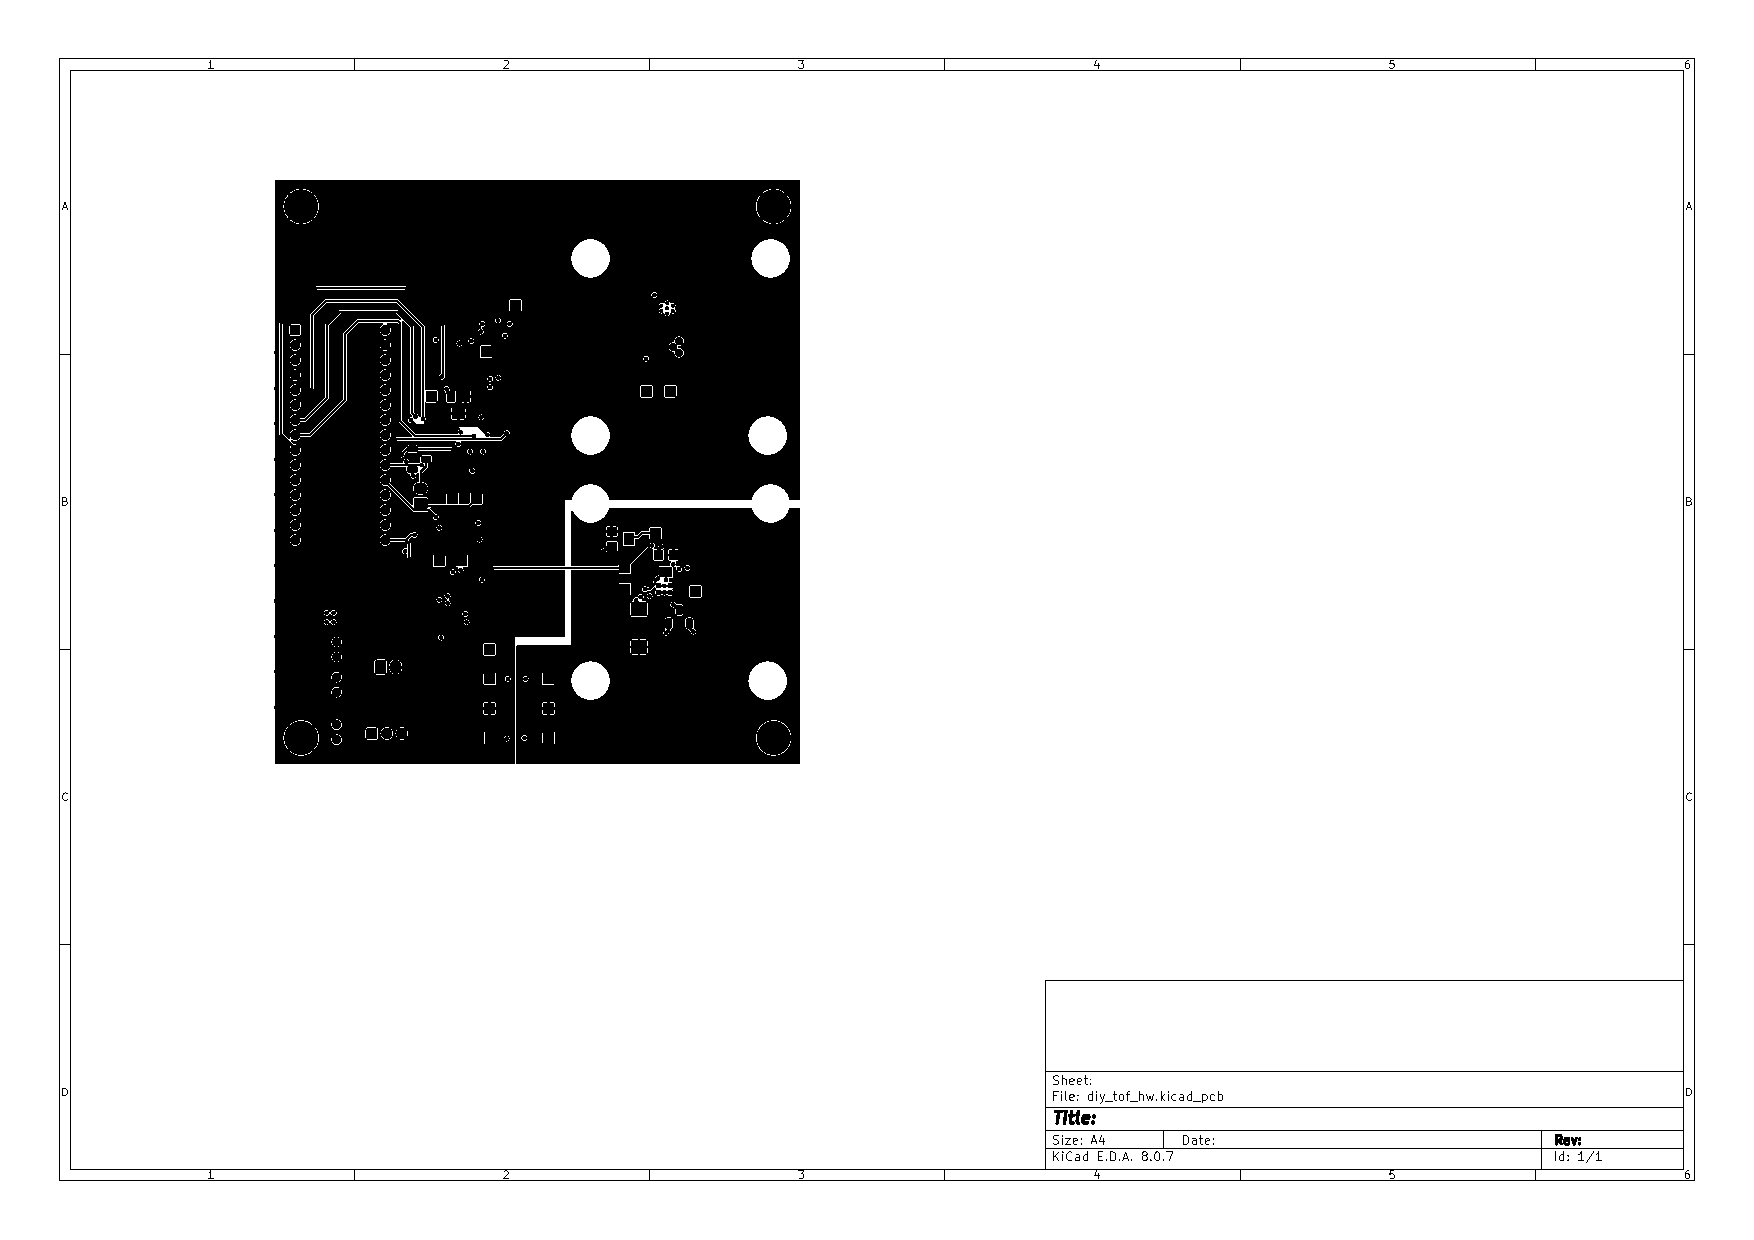
\includegraphics[trim=130 220 450 80, clip, width=0.6\textwidth]{attachments/pcb_B_Cu.pdf}
    \caption{PCB Layout Bottom}\label{fig:pcb_b_cu}
\end{figure}

\begin{figure}[H]
    \centering
    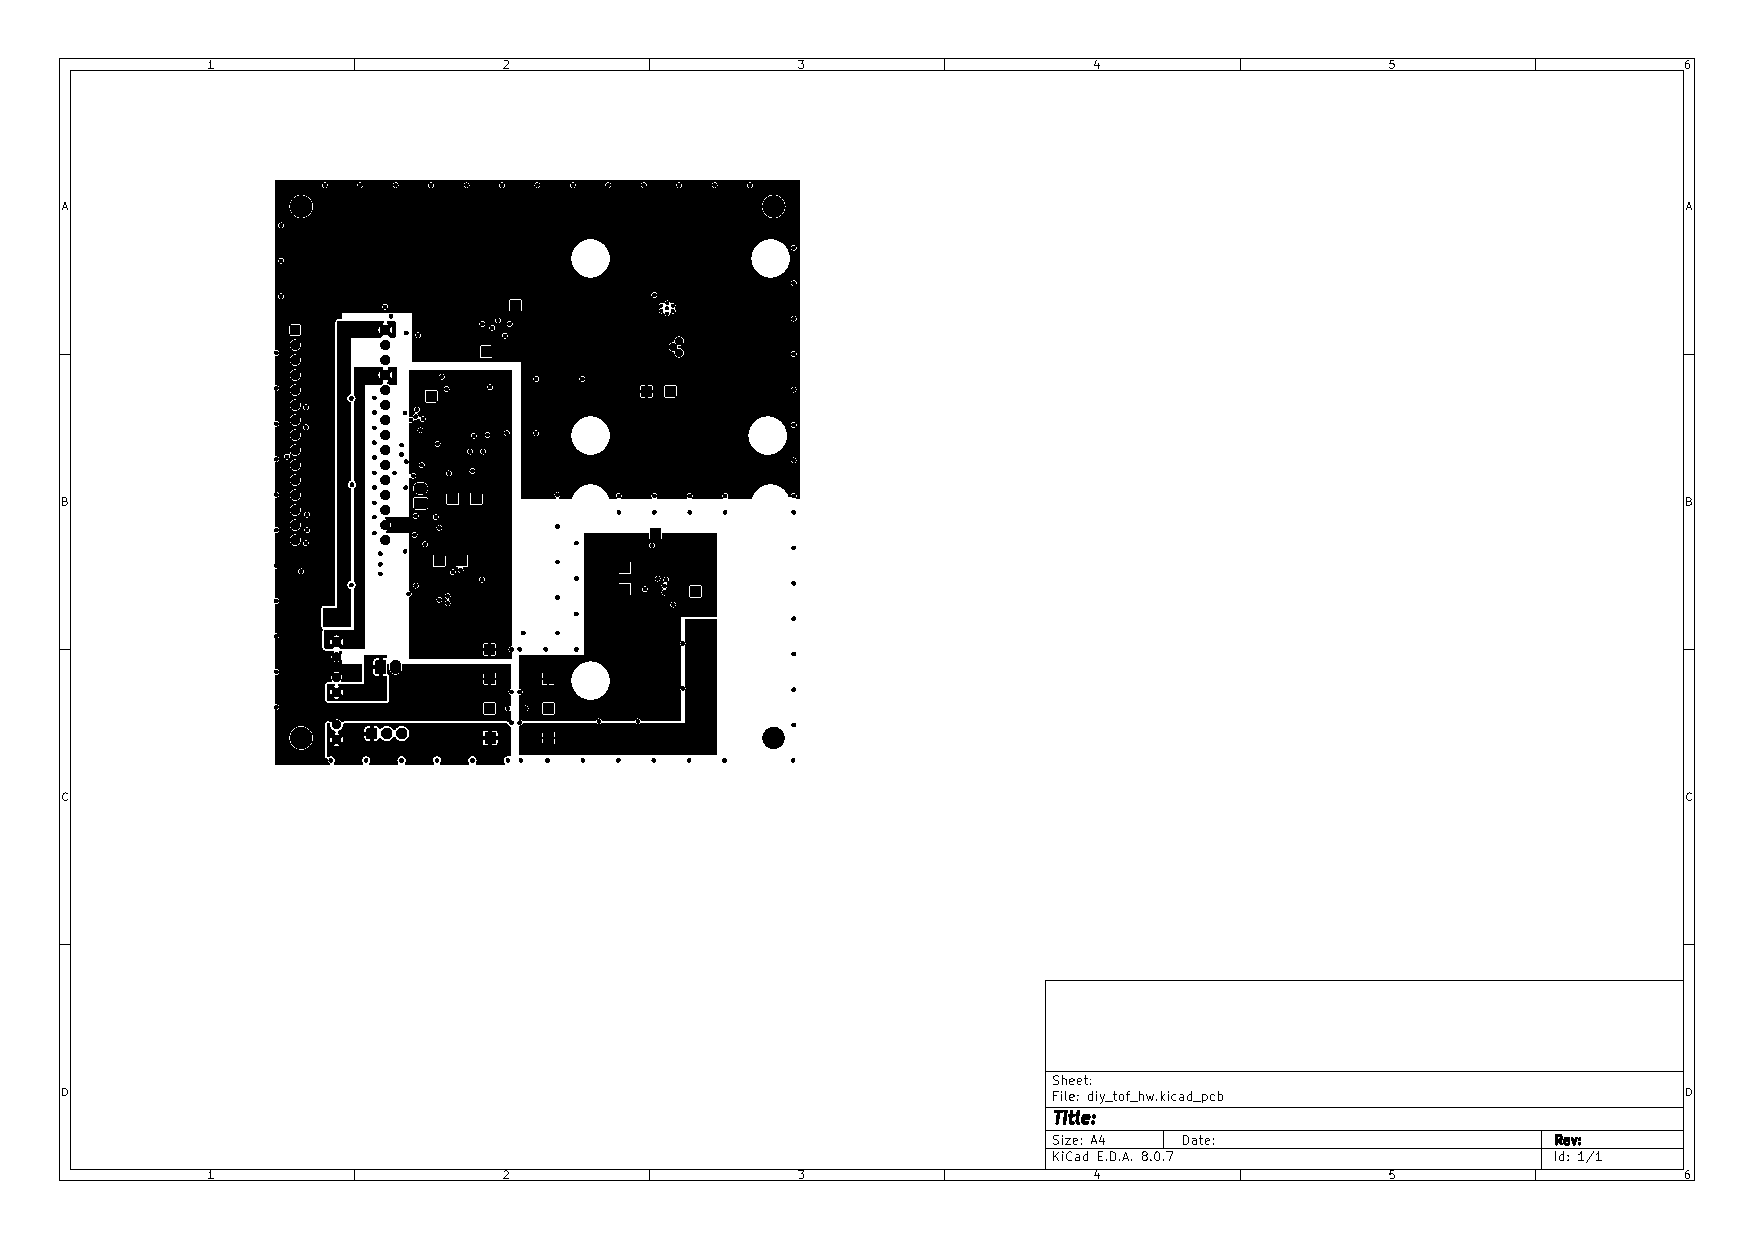
\includegraphics[trim=130 220 450 80, clip, width=0.6\textwidth]{attachments/pcb_In1_Cu.pdf}
    \caption{PCB Layout Innen 1}\label{fig:pcb_in1_cu}
\end{figure}

\begin{figure}[H]
    \centering
    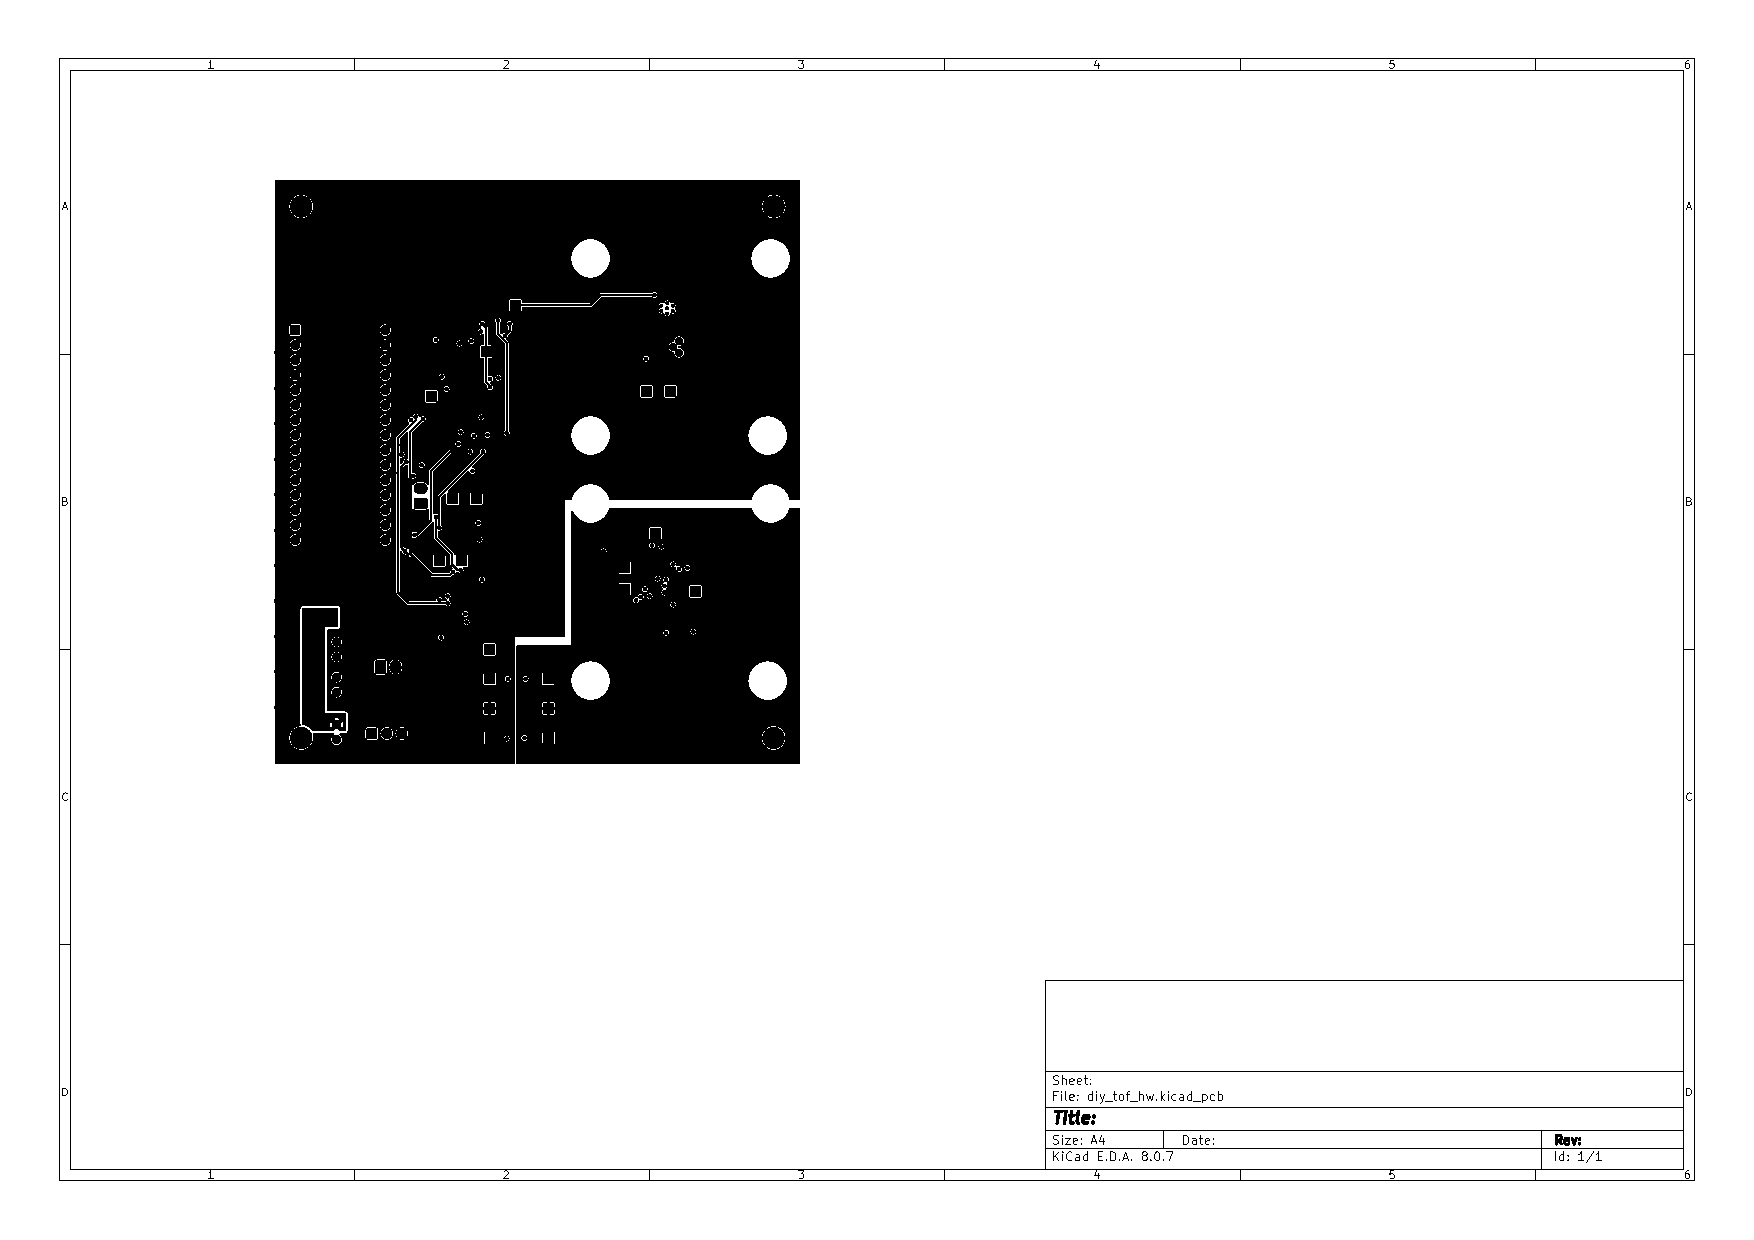
\includegraphics[trim=130 220 450 80, clip, width=0.6\textwidth]{attachments/pcb_In2_Cu.pdf}
    \caption{PCB Layout Innen 2}\label{fig:pcb_in2_cu}
\end{figure}

\subsubsection{Komponenten-Platzierung}

\begin{figure}[H]
    \centering
    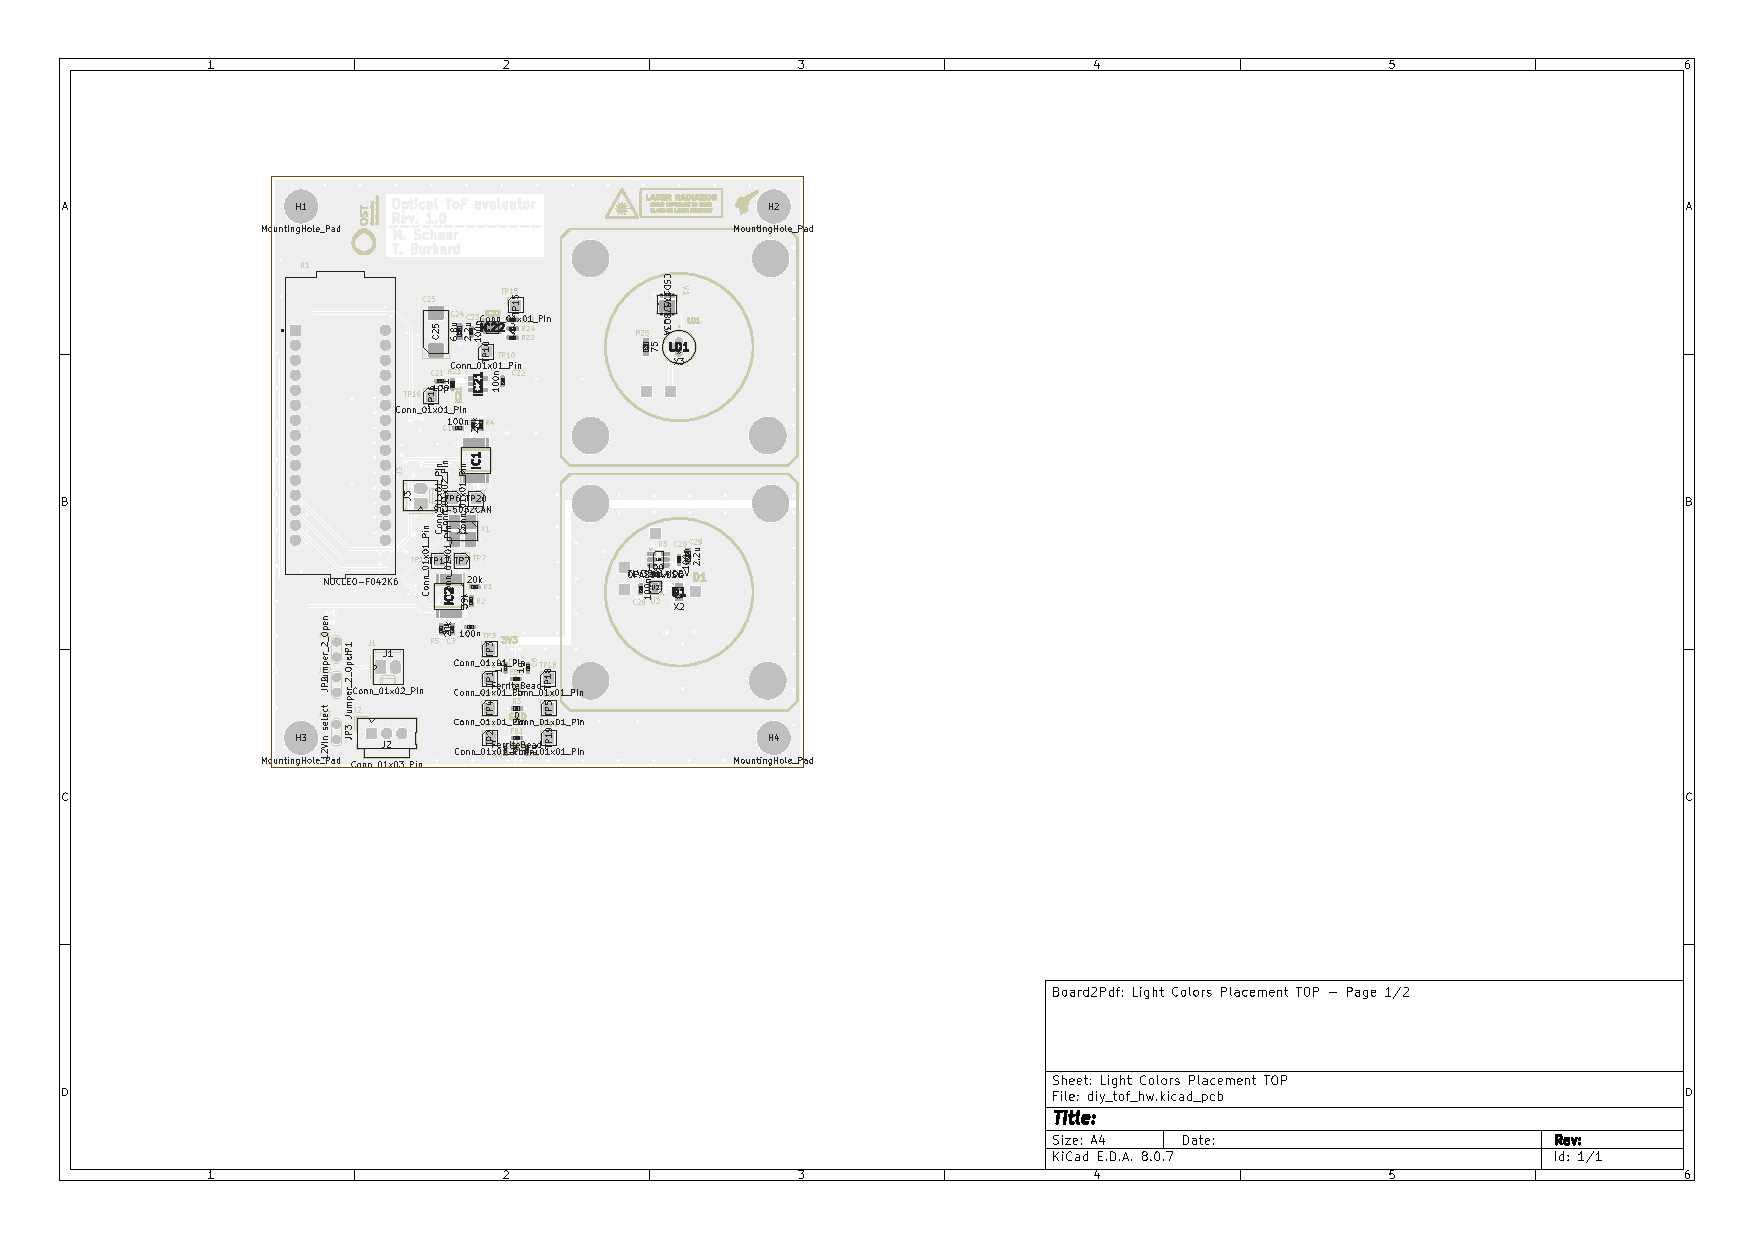
\includegraphics[page=1, trim=120 220 450 80, clip, width=0.6\textwidth]{attachments/pcb_placement.pdf}
    \caption{PCB Komponenten-Platzierung Top}\label{fig:pcb_placement_1}
\end{figure}

\begin{figure}[H]
    \centering
    \includegraphics[page=2, trim=450 220 120 80, clip, width=0.6\textwidth]{attachments/pcb_placement.pdf}
    \caption{PCB Komponenten-Platzierung Bottom}\label{fig:pcb_placement_2}
\end{figure}

\pagebreak

\subsection{3D View}

\begin{figure}[H]
    \centering
    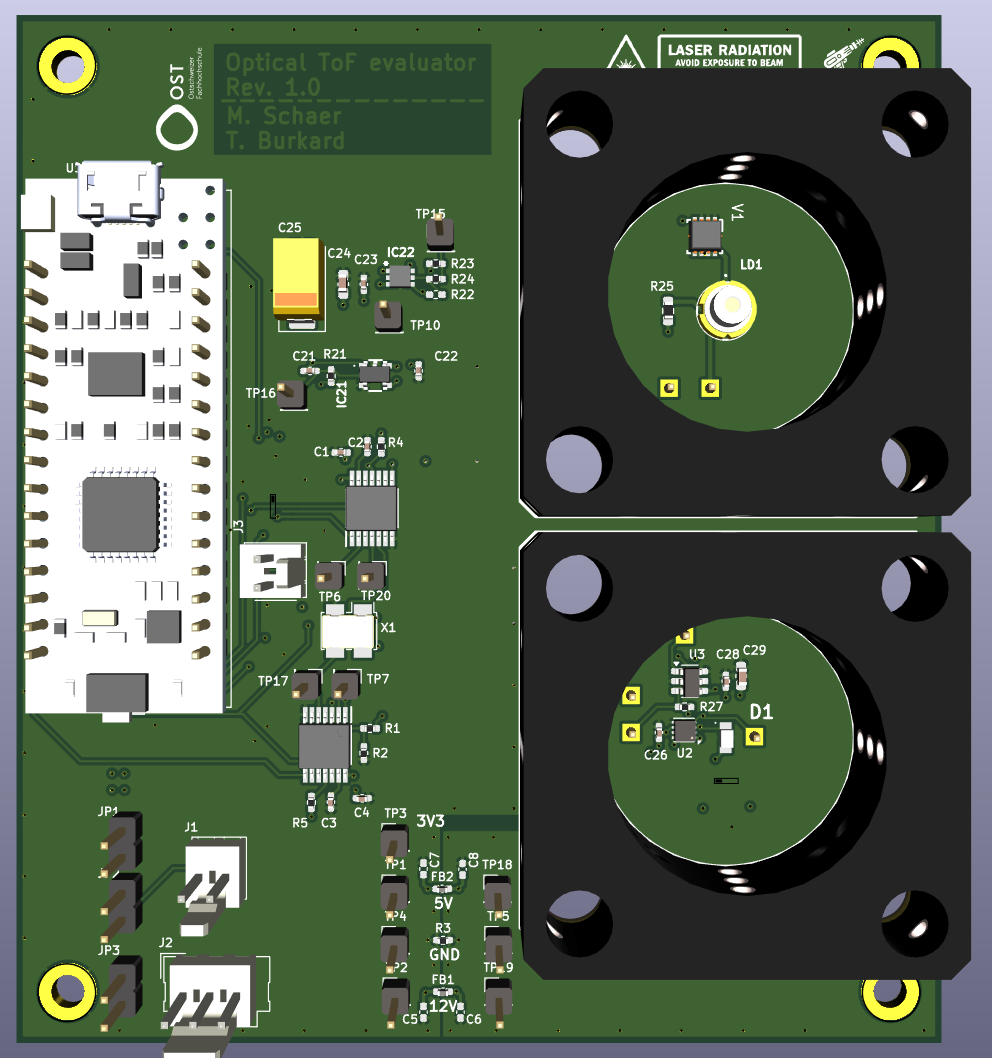
\includegraphics[width=0.6\textwidth]{graphics/3d_top.png}
    \caption{3D View Top}\label{fig:3d_top}
\end{figure}

\begin{figure}[H]
    \centering
    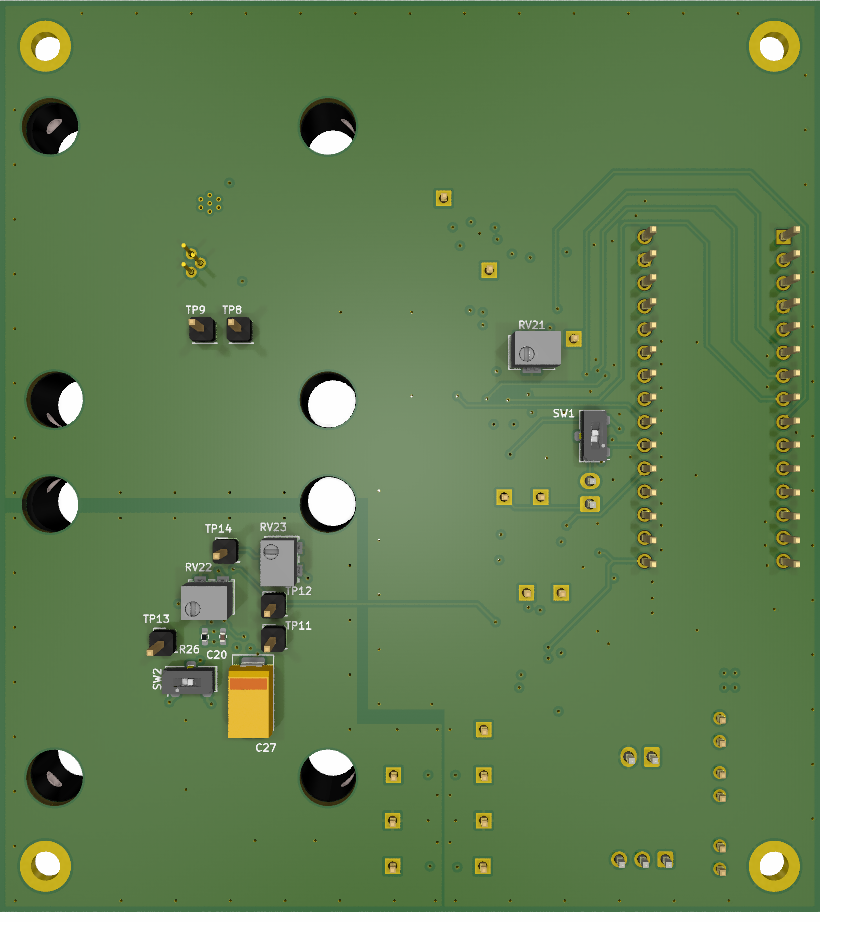
\includegraphics[width=0.6\textwidth]{graphics/3d_bottom.png}
    \caption{3D View Bottom}\label{fig:3d_bottom}
\end{figure}

\begin{landscape}

\subsection{Komponenten}

\begin{table}[H]
    \scriptsize
    \mytable
        {|l|l|l|l|l|l|}
        {\textbf{Reference} & \textbf{Value} & \textbf{Datasheet} & \textbf{Footprint} & \textbf{Qty} & \textbf{DNP}}
        {\Reference & \Value & \Datasheet & \Footprint & \Qty & \DNP}
        {tables/bom.csv}
    \caption{Bill of Material}\label{tab:bom}
\end{table}

\end{landscape}

\pagebreak

\section{Simulationen}

\subsection{Laser Treiber}
\subsection{Transimpedanzverstärker}

\pagebreak

\section{Messungen}

\pagebreak

\section{Fazit}

\pagebreak

\section{Anhang}

%%%%%%%%%%%%%%%%%%%%%% CONTENT END %%%%%%%%%%%%%%%%%%%%%%

\pagebreak

\section*{Quellenverzeichnis}
\begin{flushleft}
\begingroup
\vspace{-25pt}
\renewcommand\refname{}
\renewcommand{\addcontentsline}[3]{} % Do not add bibliography to table of contents, as there is a separate subsection "Quellenverzeichnis"
\bibliography{references}
\endgroup
\end{flushleft}


\end{document}
